\section{Research Plan}
% \begin{figure}[tbh]
% 	\begin{center}
% 		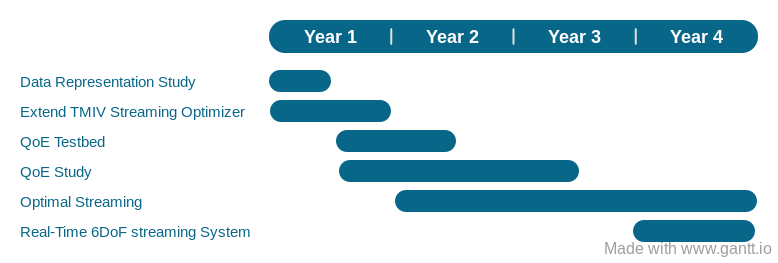
\includegraphics[width=.5\textwidth]{fig/gantta}
% 		\caption{Gantt chart of research plan.}
% 		\label{fig:Gantt}
% 	\end{center}
% \end{figure}
\begin{figure}[tbp]
	\begin{center}
	\begin{ganttchart}[y unit title=0.4cm,
	y unit chart=0.5cm,
	vgrid,hgrid, 
	title label anchor/.style={below=-1.6ex},
	title left shift=.05,
	title right shift=-.05,
	title height=1,
	bar/.style={fill=gray!50},
	incomplete/.style={fill=white},
	progress label text={},
	bar height=0.7,
	group right shift=0,
	group top shift=.6,
	group height=.3,
	group peaks={}{}{.2}]{1}{8}
	\gantttitle{Year 1}{2}
	\gantttitle{Year 2}{2}
	\gantttitle{Year 3}{2}
	\gantttitle{Year 4}{2} \\

	\ganttbar{Data Representations}{1}{1} \\
	\ganttbar{Extend TMIV Streaming Optimizer}{1}{2} \\
	\ganttbar{QoE Testbed}{2}{3} \\
	\ganttbar{User Study}{2}{6} \\
	\ganttbar{Optimal Streaming}{3}{8} \\
	\ganttbar{Real-Time 6-DoF Streaming System}{7}{8} \\
	\end{ganttchart}
	\end{center}
	\caption{Gantt Chart}
	\label{fig:Gantt}
\end{figure}

Fig.~\ref{fig:Gantt} gives the Gantt chart of my research plan.
The first problem is the data representation study.
The outcome of this research problem is our better understanding on the immersive video streaming systems, which is also useful to the research community.
Concurrently, We extend our recent work \cite{mm20_tr} to turn it into a journal paper.
After that, we work on the QoE study. We plan to build an immersive video streaming testbed and
conduct a series of user studies to understand the user experience.
We will also continue optimizing the immersive video streaming testbed by applying different optimization algorithms developed by us.  
The results of QoE study can also help us better optimize the testbed.
Last, we will design, build, and evaluate a real-time immersive video streaming system based on the results of our research 
to turn it into a journal paper.
% XXX add gantt chart at here XXX